
\documentclass[%
 reprint,
 amsmath,amssymb,
 aps,
]{revtex4-1}

\usepackage{graphicx}% Include figure files
\usepackage{dcolumn}% Align table columns on decimal point
\usepackage{bm}% bold math
\usepackage{gensymb}
\usepackage{caption}

\usepackage[implicit=false]{hyperref}
\hypersetup{
    colorlinks=true,
    linkcolor=blue,
    filecolor=magenta,      
    urlcolor=cyan,
}


\bibliographystyle{apsrev4-1}

\begin{document}



\title{Economic Effects of Natural Disasters}% Force line breaks with \\
%\thanks{A footnote to the article title}%

\author{Kaitlin Salyer}
 \affiliation{Boston University Physics Department \\
590 Commonwealth Ave.,
Boston, MA 02215 }%Lines break automatically or can be forced with \\

\date{04 May 2020}

\begin{abstract}

In 2005, the American Gulf Coast was rocked by Hurricane Katrina. It had innumerable direct and indirect impacts on the local and federal economies. Similarly, in 2011, Japan suffered the Triple Disaster: an earthquake, which caused a tsunami, which triggered a series of meltdowns at Fukushima Daiichi Nuclear Power Plant. This research intends to outline, specifically, the most impactful economic effects of these disasters, to compare and contrast the two cases, and to review the recovery methods that each country used to rebuild and re-stimulate the economy.\\

\begin{center}
	Please find related materials in my github repository:
	\url{https://github.com/ksalyer/py538}
\end{center}

\end{abstract}

\maketitle


\section{\label{sec:level1}Introduction}

Hurricane Katrina and Fukushima's earthquake (and subsequent nuclear power-plant meltdown)--each are disasters which had profound impacts on humanity. These impacts are varied, but arguably, none are more powerful or broader than the effects on the local and national economies where these disasters occurred. As will be shown in this research, the destruction caused by these disasters had both direct and indirect financial impacts. Direct economic impacts are defined as damage to or destruction of assets as a result of the disaster. Indirect economic impacts refer to the changes in the economy in the time after the disaster. ``Examples of direct economic losses include the destruction of residences, businesses, productive capital, infrastructure, crops, livestock, and (monetized) physical and mental health impacts. [... Indirect impacts] include interruptions of economic activities as well as any positive spillover effects due to the substitution of production and the demand for reconstruction" \cite{BotzenPaper}. For the purposes of this paper, we will measure these impacts on the regions of New Orleans, Louisiana (and sometimes the broader Gulf Coast) and Japan by studying the changes to their Gross Domestic Product (GDP) and their unemployment rates in the time surrounding their respective natural disasters.

\section{\label{sec:level1}Hurricane Katrina: 2005}

On August 23, 2005, a tropical depression arose over the Bahamas. Over the next two days, this storm gained strength and made landfall in Florida. By this point it was a category 1 hurricane. As the hurricane moved over the Gulf of Mexico, it greatly intensified, reaching category 3 status. Hurricane Katrina made its way to Louisiana on August 29, 2005 as a category 4 hurricane. Much of New Orleans is below sea level, and they had previously installed a levee system in an effort to prevent massive flooding; however, after Hurricane Katrina passed by New Orleans, the nearby lake overflowed. The levees breached. The storm struck in the morning of August 29, but by the afternoon, approximately 20\% of the city was underwater. By August 30, about 80\% of the city was underwater. Tens of thousands of residents took up shelter in the local convention center and the Louisiana Superdome. Food supplies and potable water were running short. Severe looting occurred in some neighborhoods. Local aid was unable to help as their buildings and resources were flooded as well; thus, it became the responsibility of national organizations to aid and rescue the people of New Orleans. In the end, Hurricane Katrina took rank as the costliest natural disaster in United States history. \cite{Katrina_encyclopedia}

\subsection{\label{sec:level2} Social and Economic Context}

Before considering the direct damage and the potential for recovery of New Orleans from this disaster, it is important to first address the social and economic context of the area before the devastation. New Orleans was already in a decline before Katrina struck:  ``Its peak of relative importance was in 1840, when six of every thousand residents of the United States lived in the city. Its absolute population peak occurred in 1960" \cite{VigdorPaper}. The cause of this decline can be attributed to the fact that New Orleans' draw was once its identity as a river port, but with the rise of other modes of transportation and distribution of goods and services (and the costly difference between traveling upstream versus downstream), river barges were rendered rather obsolete. Thus, as time went on, the city was less appealing to manufacturers and businesses. Since then, New Orleans' population grew with the rest of the U.S., but it has not been as booming or as large of a contributor the overall U.S. population since 1840. \cite{VigdorPaper}

As such, the local economy began to depend more and more heavily on tourism, and the leading industries in terms of employment in the area became entertainment, accommodation, and food services; transportation, warehousing, and utilities; and public administration \cite{VigdorPaper}. Using the 2000 Census data (Table \ref{NOLA_table}) as a snapshot of pre-Katrina New Orleans, the city had higher rates of unemployment and poverty, a lower median income, and a larger percentages of adults over 25 without a high school diploma than the national averages. From this data, it is clear to see that New Orleans was already in a state of decline before Hurricane Katrina struck.

\begin{table*}[]
\caption{Labor Market Statistics for New Orleans Metropolitan Area and United States, 2000 Census}
\begin{tabular}{|l|c|c|}
\hline
 & New Orleans Metropolitan Area & United States \\ \hline
Labor force participation rate, persons age 16 and over  & 61.2\%  & 63.9\%        \\ \hline
Unemployment rate & 4.1\%  & 3.7\%         \\ \hline
\begin{tabular}[c]{@{}l@{}}Proportion of employed persons working at least\\ 35 hours/week, at least 50 weeks/year\end{tabular} & 57.8\% & 58.3\%        \\ \hline
Proportion of households with wage or salary income  & 76.9\% & 77.7\%        \\ \hline
Median household income in 1999  & \$35,517  & \$41,994      \\ \hline
Poverty rate  & 18.4\%  & 12.4\%        \\ \hline
Percent with income below 50\% of the poverty line & 9.3\%  & 5.6\%         \\ \hline
Percent of adults over 25 without a high school diploma  & 22.3\% & 19.6\%        \\ \hline
\end{tabular}
\caption*{Table reproduced from \cite{VigdorPaper}}
\label{NOLA_table}
\end{table*}

\subsection{\label{sec:level2} Direct Impacts}

One of most critical direct impacts of Hurricane Katrina on the local and national economy was its evacuation or destruction of oil platforms and pipelines in the Gulf of Mexico. The storm destroyed 46 platforms and damaged 100 pipelines. The gargantuan waves sunk entire platforms or snapped the anchors, leaving the platforms adrift \cite{Katrina_oil}. Ultimately, this resulted in damage to 19\% of the United States' oil production \cite{Katrina_oil_balance}. The production lines further suffered when Hurricane Rita passed through almost exactly the same path about a month later. These two storms had very similar effects on the oil and natural gas industries, and their impact is often reported combined. As such, these two hurricanes threatened 47 major natural gas processing plants and 17 natural gas liquids fractionation sites along the Gulf Coast \cite{Katrina_naturalGas}.

As participants in the information age (even fifteen years ago), we often forget just how essential our communications infrastructure in supporting the daily functions of our society. Hurricane Katrina exposed this when it obliterated the local communications system. ``Over 180 central office locations were running on generators as commercial power sources failed. About 100 commercial radio stations were forced off the air. Up to 2,000 cell towers were also knocked out and responder Land Mobile Radio communications were significantly degraded. Energency 911 service was severely damaged, and surviving stations were soon overwhelmed by spiking call volumes as desperate people tried to get help or check on those at risk" \cite{MillerPaper}. The failures of the communications system had a cascading effect: several other systems and resources failed due to unreliable or nonexistent cellular, internet, or electrical connections.

A third direct impact to the local industries and economy happened in the agriculture sector. While there was not a severe national impact on Gulf Coast crops, the ability of this industry to export was greatly impacted. In 2004, 22\% of national wheat exports, 71\% of corn exports and 65\% of soybean exports were handled in Gulf ports, but this was not possible in the time immediately following the devastation of Katrina. It would not be until late in the fall of that year that the ports were again operational. \cite{samuelson_2005} It serves to note that, while New Orleans garnered significant amounts of media attention at the time due to the sustained flooding, it was not the only community devastated by Hurricane Katrina. Neighboring state Mississippi also suffered major damages to their agriculture and forestry industries. Gulfport, Mississippi's major ocean shipping port was shutdown for almost a year, meaning businesses such as Chiquita and Dole, who had significant presence in this port, had to find different ports to use. Furthermore, forestry, which is a major industry in southern Mississippi in particular, experienced damage to 1.3 million acres of forestland due to Hurricane Katrina. It is estimated that 14.5 million cords of paperwood and 3.2 billion board feet of sawtimber were destroyed, leading to an estimated \$1.1 billion in damages. \cite{grizzard_2005}

There was also severe damage to utilities and their providers. Entergy Corporation defines themselves as, ``an integrated energy company engaged primarily in electric power production and retail distribution operations" \cite{entergy}. Their market is primarily in the Deep South, and their company is headquartered in New Orleans. During the hurricane, they lost 1,763 distribution poles, about half of their substations were flooded, and 76\% of their transmission lines went out of service. 65\% of their customers were unable to accept services due to damages to homes and businesses. About a month after Katrina hit the Gulf Coast, the New Orleans branch of Entergy filed for bankruptcy protection. The company noted the causes as decreased revenue and approximately \$1 billion in restoration costs. \cite{walton_2015}

Of course, all of these damages to infrastructure and business assets cost a lot of money to rebuild and recover. This destruction was supplemented with damages to residential and private properties and many local, small businesses. Much of the money used to rebuild New Orleans came in the forms of insurance and government aid, but there were plenty of instances of businesses and individuals being forced to pay out-of-pocket to restore what was lost. Furthermore, each of these direct impacts of the storm had reverberating indirect negative impacts on the economy. 

\subsection{\label{sec:level2} Indirect Economic Impacts}

Perhaps the most crucial indirect economic impacts of Hurricane Katrina were those pertaining to the oil and gas industries. The Gulf of Mexico was, at the time, the source of 30\% of United States' oil production and 24\% of United States' natural gas; however, several companies such as Exxon Mobil and Chevron had to close operations before the storm raged through the Gulf. \cite{laverty_2005} Many companies had to remain closed in the time following the passage of Katrina because of repairs or simply because employees were not able to work. Once 95\% of the Gulf's oil production and 88\% of its natural-gas output were shut down, the cost of gasoline rose to \$6 a gallon in the South. Nationally, the gas prices rose quickly and stayed high (above \$3 a gallon) to renormalize, rebalance the supply and demand. The increase in expenditures on fuel and gas for heating homes meant consumers were more restrictive in their non-essential spending habits. \cite{samuelson_2005} 

As discussed in the previous section, the destruction of the communication infrastructure led to a cascading effect on other important systems. Perhaps the most difficult problem, however, was the difficulty it added to organizing aid and recovery missions. ``Also--and very importantly--the lack of authoritative and believable information from public officials created a climate rife with rumor, misinformation and speculation, significantly reduced the government's ability to maintain public order, and added to the sense of dislocation and loss of public confidence" \cite{MillerPaper}. Essentially, due to lack of effective, reliable communications, there was a degree of civil unrest, an increase in crime. Many survivors resorted to riots and looting. These incidents added to the overall damages suffered by businesses.

The sum total of the destruction had a dramatic effect on the local GDP. As shown in Figure \ref{fig:NewOrleans_GDP}, between 2001 and 2005, the GDP of New Orleans was increasing significantly. When Katrina hit, the GDP plateaued for that year and began to increase again like it did before the hurricane. This stagnation is likely due to the combination of reduced income to both individuals and businesses, a large migration out of the city, and the large amounts of money spent on rebuilding. Furthermore, there was a steep increase in the unemployment rate in the New Orleans metro-area (see Figure \ref{fig:NewOrleans_unemployment}). Unemployment peaked in the month after Katrina because businesses were shut down and large portions of the population were displaced. Unemployment was rampant in the oil and natural gas industries, the entertainment and tourism industries, and shipping industries in particular.

\begin{figure}
	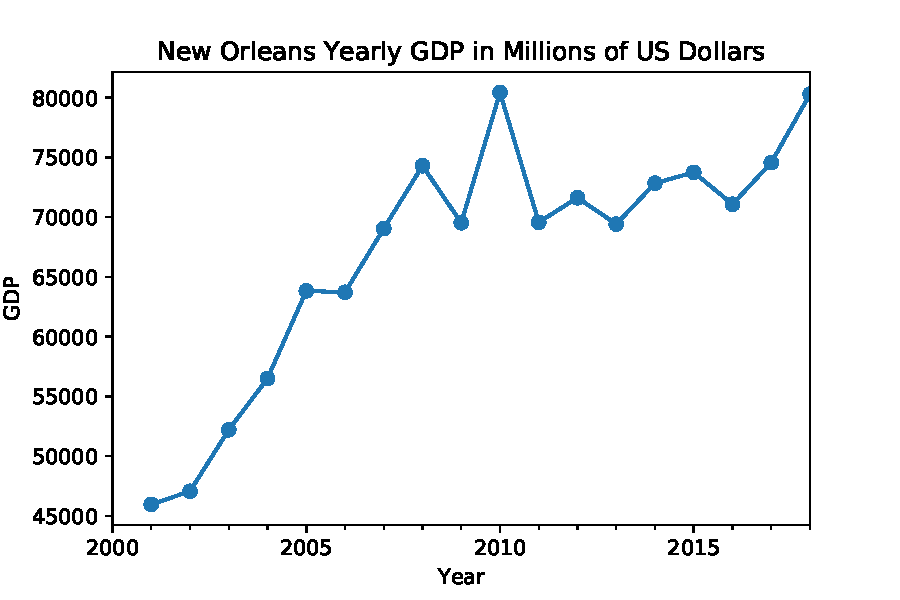
\includegraphics[scale=0.6]{plot_NewOrleans_GDP.pdf}
	\centering
	\caption{Plot showing the GDP of New Orleans, Louisiana, measured yearly and in millions of US dollars. Data sourced from Federal Reserve Bank of St. Louis \cite{NOLA_GDP_data}.}
	\label{fig:NewOrleans_GDP}
\end{figure}

\begin{figure}
	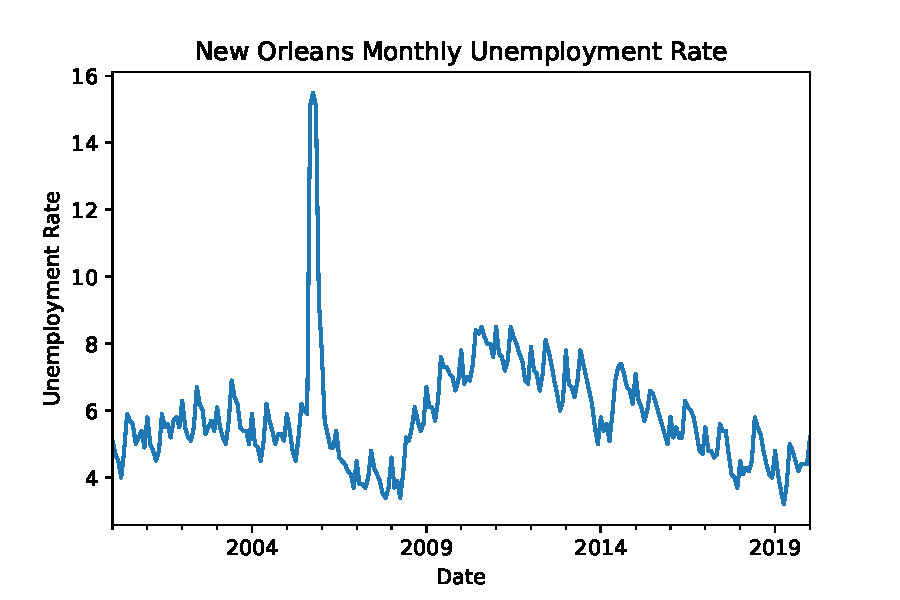
\includegraphics[scale=0.6]{plot_NewOrleans_unemployment.pdf}
	\centering
	\caption{Plot showing the unemployment rate of New Orleans, Louisiana, measured monthly. Data sourced from Federal Reserve Bank of St. Louis \cite{NOLA_unemployment_data}.}
	\label{fig:NewOrleans_unemployment}
\end{figure}

\subsection{\label{sec:level2} Recovery Methods}

Even now, New Orleans is still working to get back to its pre-Katrina heights; however, the city has grown and recovered beautifully in the last fifteen years. The unemployment rate is averaging about the same as pre-Katrina days and its population is returning as well. In fact, New Orleans is one of the United States' fastest growing cities. The local GDP has also grown significantly, in spite of the fact that the country faced the Great Recession not long after Katrina. This can also be seen in Figure \ref{fig:NewOrleans_GDP}.

A significant portion of this rebuilding and growth came at the hands of federal aid. The Federal Emergency Management Agency (FEMA) contributed \$120.5 billion and federal block grants contributed \$247.5 million to rebuild the Gulf Region and its schools. Businesses were stimulated using funds from small business loans, Department of Commerce investment, and the community renewal efforts of Housing and Urban Development (HUD) and the Internal Revenue Service. The Department of Labor gave more than \$350 million to bolster and develop the regional workforce. Other organizations such as the Army Corps of Engineers, NOAA, FEMA, the Coast Guard, and the Environmental Protection Agency aided in environmental cleanup and restoration. All of this has served to make New Orleans more independent over the years, drawing in \$7 billion in capital investment in the span of five years on its own. This entices startups and young professionals, meaning the city will continue to grow and thrive. \cite{meys_franzi_2018}

Given the cost of rebuilding New Orleans and the rest of the Gulf Coast, it became very clear to the various levels of the United States government that preparation is key to prevent many of the mistakes that were made in response to Katrina. In particular, communities have already or are currently planning strategies that are flexible but still target how to respond in the event of a disaster like Katrina. This is known as the Comprehensive Economic Development Strategy (CEDS) and the purpose is, ``to anticipate risks, evaluate impact on the economy, and build equitable response measures to avoid the disruption or to mitigate effect" \cite{meys_franzi_2018}. CEDS provides a framework to build economic resilience. This includes, ``identifying persistent economic challenges or deficiencies, preparing for disruption by identifying `early-warning' tools, building mechanisms that create flexibility, and promoting a positive vision for the region" \cite{meys_franzi_2018}. This allows communities to prepare for a potential disaster by allocating resources before they become necessary and increasing coordination and efficiency between agencies to minimize response times.

\section{\label{sec:level1}Fukushima Nuclear Disaster: 2011}

On Friday, March 11, 2011, a massive, 9.0 magnitude, undersea megathrust earthquake occurred off the east coast of Japan. The loss of life and damage from this earthquake was minimal due to Japan's investment in earthquake-resistant engineering. \cite{ferris_2013} It did, however, trigger a tsunami with waves over a hundred feet tall, traveling at 435 miles per hour towards Japan. Residents had mere minutes to find safety from the incoming waves. \cite{buerk_2011} Japanese authorities reported more than 120,000 buildings collapsed entirely and more than a million others were half-collapsed or partially damaged throughout the country. \cite{npa_2020} The event which caused the most fear and damage, however, was the subsequent series of meltdowns at the Fukushima nuclear power plant. Fukushima's nuclear disaster was the worst since Chernobyl in 1986, and the three events together--known as the Triple Disaster--are the most expensive disasters in human history. \cite{ferris_2013}

\subsection{\label{sec:level2} Social and Economic Context}

At the time that the earthquake occurred, Japan was the third-largest economy in the world, and its GDP accounted for 8.7\% of the global GDP. However, in the decades preceeding the event, Japan's growth rate was slow in comparison with the world as a whole and thus was not a major contributor to global economic growth. The country also held a very important position in the world economy in terms of production lines and supplying materials for automobiles, semiconductors, and electronics. Before the Triple Disaster the yen was strengthening in value. \cite{nanto_2011} 

\subsection{\label{sec:level2} Direct Economic Impacts}

The most serious and direct economic impact of the earthquake and the tsunami is the series of meltdowns at the Fukushima Daiichi Nuclear Power Plant. While the plant had emergency failsafes in place in case of an earthquake which operated as planned, the tsunami came about an hour later, breaching the seawall and flooding the emergency backup generators used for the cooling system. When these failed, the fuel of the nuclear reactor continued to give off heat which eventually caused a meltdown. This happened in four of the 6 reactors. There were also hydrogen explosions that occurred as operators attempted to release pressure in the reactors. The escape system for these gases had several leaks. When the hydrogen built up and reacted with the surrounding oxygen, there were significant explosions in three of the reactors. \cite{youtube_2012} The cost associated with decommissioning and decontaminating the area, in addition to paying out compensation to plaintiffs in lawsuits and storing radioactive waste, has been estimated to be \$187 billion. The process of decommissioning the plant, however, will take at least 40 years, so it is possible that this estimate is still too low. Furthermore, it is estimated that \$21 billion of the total cost will be passed to consumers in the form of higher energy and electricity bills. \cite{mccurry_2017}

Japan holds an essential place in the world's manufacturing industry. Not only are they the home of a number of companies which build and export electronics, but also they are suppliers for other Asian countries, such as China, who export a vast range of goods around the world. When the Triple Disaster occurred, several large and notable companies such as Hitachi, Renesas Electronics, NEC, Sony, and Fujitsu had to shut down operations in affected regions. Several ports were also damaged and unable to be used. These shutdowns stalled production lines and the imports and exports of goods, echoing the problems faced in the Gulf Coast after Hurricane Katrina. Furthermore, it had a small but noticeable effect on Japanese-owned companies in the United States. For example, Toyota, Mitsubishi, Nissan, and Mazda production lines in the United States also stalled as they waited for the import of engines and transmissions from Japan. \cite{nanto_2011}

There were additionally significant damages to the country's agricultural, forestry, and fishing industries, but these accounted for less than 5\% of the country's GDP. They imported more products in these industries than they exported. \cite{nanto_2011} Of course, as with any large disaster, there was significant loss of personal and private property of individuals and small businesses. However, in this particular case, there were about 160,000 people forced to evacuate the area surrounding the Fukushima power plant, unlikely to be allowed to return home due to the dangers associated with continued radiation. \cite{mccurry_2017}

\subsection{\label{sec:level2} Indirect Economic Impacts}

Japan invested in building nuclear power plants to avoid importing large amounts of fossil fuels, as this is expensive and the country has limited access to these natural resources otherwise. With the shutdown of Fukushima Daiichi and the public outcry against nuclear power, Japan had to resort to increasing their import of fossil fuels. Their imports of these resources increased between 2010 and 2012 by almost \$60 billion. \cite{harlan_2012} ``The damage, furthermore, has been compounded by the nuclear contamination from the Fukushima Daiichi Nuclear Plant plus a shortage of gasoline and of electricity that has caused rolling blackouts in Japan's industrial centers" \cite{nanto_2011}. There were several companies who could not carry out production or continue business due to conservation of energy resources for essentials only. This problem persisted months later: businesses and the public were asked to conserve power as much as possible through the summer months \cite{rubin_2011}.

The country being low on power hampered industrial production and decreased exports at the same time that expensive imports were rising, leading to the stagnation in the country's GDP as seen in Figure \ref{fig:Japan_GDP}. Before the Triple Disaster, Japan was doing fairly well for itself, even in spite of the global recession in 2008 and 2009. Their GDP was gradually increasing until 2011, where it stalled before starting a downward trend for the country. It has, since 2015 started to recover, but is still not close to pre-2011 status. Interestingly, the national unemployment rate, as shown in Figure \ref{fig:Japan_unemployment}, didn't have a particularly shocking change. Unemployment for the country has been in a downward trend since 2009.

\begin{figure}
	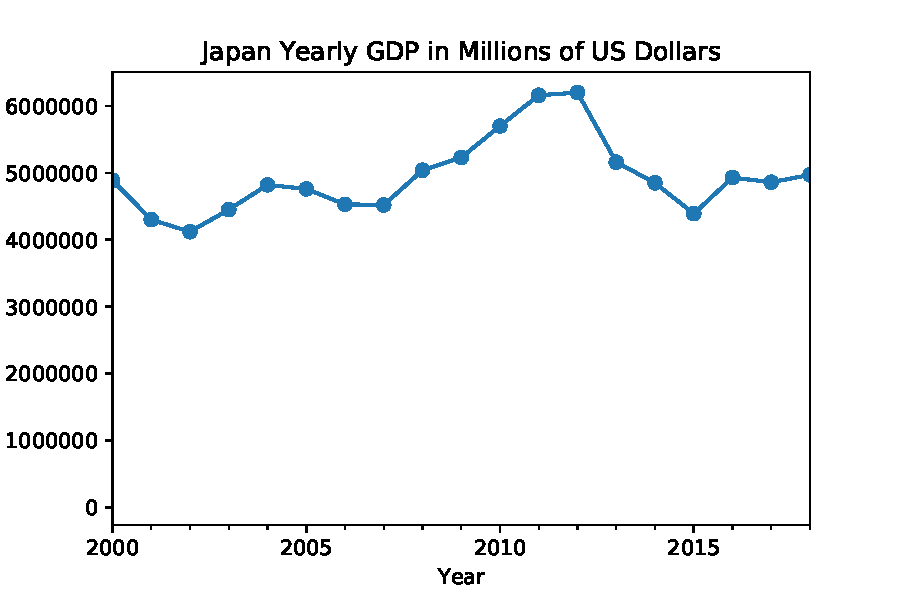
\includegraphics[scale=0.6]{plot_Japan_GDP.pdf}
	\centering
	\caption{Plot showing the GDP of Japan, measured yearly and in millions of US dollars. Data sourced from Federal Reserve Bank of St. Louis \cite{JPN_GDP_data}.}
	\label{fig:Japan_GDP}
\end{figure}

\begin{figure}
	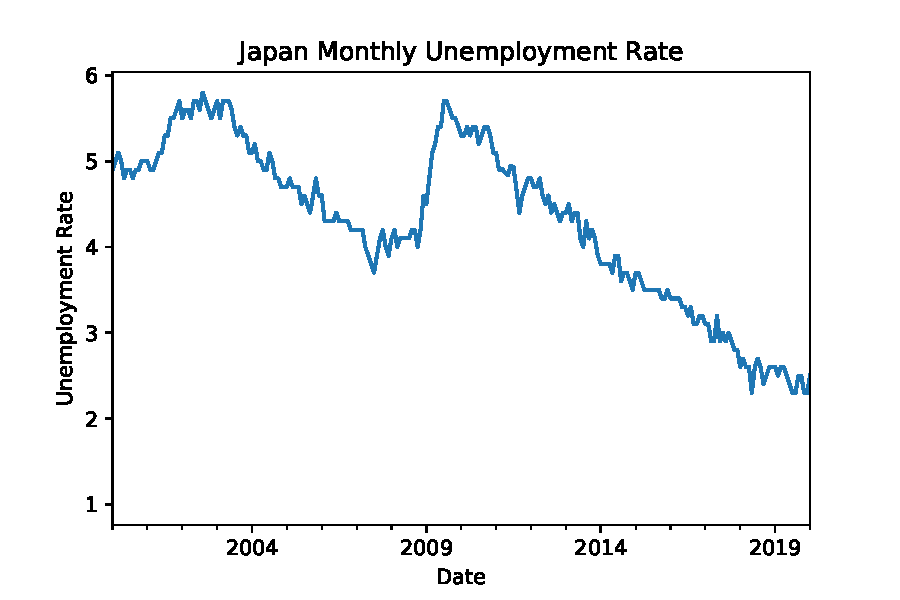
\includegraphics[scale=0.6]{plot_Japan_unemployment.pdf}
	\centering
	\caption{Plot showing the unemployment rate of Japan, measured monthly. Data sourced from Federal Reserve Bank of St. Louis \cite{JPN_unemployment_data}.}
	\label{fig:Japan_unemployment}
\end{figure}

\subsection{\label{sec:level2} Recovery Methods}

Initial responses to the crisis included the Bank of Japan providing liquidity in hopes of stabilizing markets. While this probably relieved some immediate pressures, the long term effects were quite harmful to the overall national economy. The value of the yen decreased, the prices of commodities were increasing, the national debt was mounting. Many thought Japanese investors may sell United States treasuries, which would have reduced the value of the dollar and made importing to the United States more expensive. Ultimately, Japan decided that would not be a worthwhile strategy and instead financed the rebuilding and recovery program through taxation. \cite{amadeo_2020}

\section{\label{sec:level1}Discussion}

2005's Hurricane Katrina striking the United States Gulf Coast and 2011's earthquake and tsunami off the Pacific Coast of Japan are two of the costliest disasters in human history. While the specific effects were different, the damage done to the affected economies was very similar. Both were left with fuel shortages to varying degrees and suffered losses to their primary industries, leading to plateaus in their GDPs in the respective years of the disasters. There was, however, a very interesting difference in the unemployment rates of both economies: New Orleans experienced a startling uptick in unemployment, whereas Japan did not. Further studies may find a relationship between 1. unemployment and 2. population and loss of life in these disasters.

In both cases, however, the recovery method was, simply put, to rebuild and stimulate the local economy using federal funds. It seems that there is no way around this as the government is the only entity that can organize that kind of effort and take on that kind of debt. The best solution is to prepare various strategies to respond to these tragedies in the most efficient and cost-effective way possible, and to keep those plans updated.

Given this, it is worth the investment into scientific and engineering research to develop new materials and resources that would help prevent as much damage as possible. Certainly the short term cost of fortifying New Orleans' levees or engineering several levels of failsafes in Japan's nuclear power plants will save governments many billions of dollars when tragedies occur. Furthermore, future economies would benefit from current funding of research into what actions can be taken to lessen the chances of gigantic disasters such as these. Humans put intense pressure on the environment, worsening climate change and causing more frequent extreme weather. This would be a very interesting study to investigate next: weighing the cost of self-preservative climate research against the cost of recovering from disasters.

\bibliography{Salyer_py538_FinalPaperBiblio}

\end{document}
%
% ****** End of file apssamp.tex ******